% Evidence path for pipe p520 (L-TOWN, seed 42), as returned by the GraphRAG retriever.
% Compile with pdflatex to fig_evidence_path.pdf. Every node is defined before any edge.
\documentclass[border=2pt]{standalone}
\usepackage[T1]{fontenc}
\usepackage{lmodern}
\usepackage{tikz}
\usetikzlibrary{positioning,arrows.meta}
\begin{document}
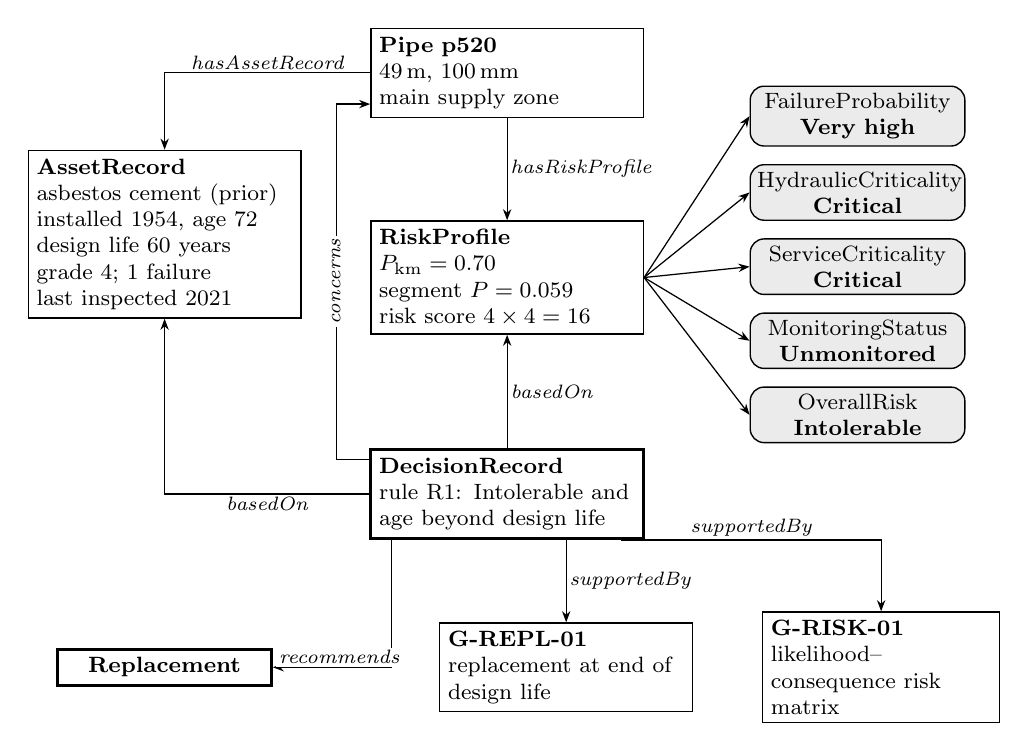
\begin{tikzpicture}[
  font=\footnotesize,
  every node/.append style={execute at begin node={\hyphenpenalty10000 }},
  ent/.style={draw=black, fill=white, line width=0.5pt, align=left, inner sep=3pt, text width=3.25cm},
  band/.style={draw=black, fill=black!8, line width=0.5pt, rounded corners=5pt, align=center,
               inner sep=2.5pt, text width=2.55cm, minimum height=0.62cm},
  key/.style={ent, line width=1.1pt},
  rel/.style={-{Stealth[length=4pt]}, line width=0.45pt},
  lab/.style={font=\scriptsize\itshape, fill=white, inner sep=1pt},
]
%% entities
\node[ent] (pipe) at (0,0) {\textbf{Pipe p520}\\ 49\,m, 100\,mm\\ main supply zone};
\node[ent] (ar) at (-4.35,-2.05) {\textbf{AssetRecord}\\ asbestos cement (prior)\\ installed 1954, age 72\\ design life 60 years\\ grade 4; 1 failure\\ last inspected 2021};
\node[ent] (rp) at (0,-2.6) {\textbf{RiskProfile}\\ $P_{\mathrm{km}} = 0.70$\\ segment $P = 0.059$\\ risk score $4 \times 4 = 16$};
\node[key] (dr) at (0,-5.35) {\textbf{DecisionRecord}\\ rule R1: Intolerable and age beyond design life};
%% shared band nodes
\node[band] (fp) at (4.45,-0.55) {FailureProbability\\ \textbf{Very high}};
\node[band, below=0.22cm of fp] (hc) {HydraulicCriticality\\ \textbf{Critical}};
\node[band, below=0.22cm of hc] (sc) {ServiceCriticality\\ \textbf{Critical}};
\node[band, below=0.22cm of sc] (ms) {MonitoringStatus\\ \textbf{Unmonitored}};
\node[band, below=0.22cm of ms] (or) {OverallRisk\\ \textbf{Intolerable}};
%% outcome
\node[key, text width=2.5cm, align=center] (act) at (-4.35,-7.55) {\textbf{Replacement}};
\node[ent, text width=3.0cm] (g1) at (0.75,-7.55) {\textbf{G-REPL-01}\\ replacement at end of design life};
\node[ent, text width=2.8cm] (g2) at (4.75,-7.55) {\textbf{G-RISK-01}\\ likelihood--consequence risk matrix};

%% relationships
\draw[rel] (pipe.west) -| node[lab, pos=0.25, above] {hasAssetRecord} (ar.north);
\draw[rel] (pipe.south) -- node[lab, right] {hasRiskProfile} (rp.north);
\foreach \b/\p in {fp/hasFailureProbability, hc/hasHydraulicCriticality, sc/hasServiceCriticality,
                   ms/hasMonitoringStatus, or/hasOverallRisk}
  \draw[rel] (rp.east) -- (\b.west);
\draw[rel] (dr.north) -- node[lab, right] {basedOn} (rp.south);
\draw[rel] (dr.west) -| node[lab, pos=0.25, below] {basedOn} (ar.south);
\draw[rel] ([yshift=-4pt]dr.north west) -- ++(-0.42,0) |- node[lab, pos=0.25, rotate=90, fill=white] {concerns} ([yshift=5pt]pipe.south west);
\draw[rel] ([xshift=8pt]dr.south west) |- node[lab, pos=0.72, above] {recommends} (act.east);
\draw[rel] (dr.south -| g1.north) -- node[lab, right] {supportedBy} (g1.north);
\draw[rel] (dr.south east) ++(-0.3,0) -| node[lab, pos=0.25, above] {supportedBy} (g2.north);
\end{tikzpicture}
\end{document}
